% Options for packages loaded elsewhere
% Options for packages loaded elsewhere
\PassOptionsToPackage{unicode}{hyperref}
\PassOptionsToPackage{hyphens}{url}
\PassOptionsToPackage{dvipsnames,svgnames,x11names}{xcolor}
%
\documentclass[
  12pt]{article}
\usepackage{xcolor}
\usepackage{amsmath,amssymb}
\setcounter{secnumdepth}{5}
\usepackage{iftex}
\ifPDFTeX
  \usepackage[T1]{fontenc}
  \usepackage[utf8]{inputenc}
  \usepackage{textcomp} % provide euro and other symbols
\else % if luatex or xetex
  \usepackage{unicode-math} % this also loads fontspec
  \defaultfontfeatures{Scale=MatchLowercase}
  \defaultfontfeatures[\rmfamily]{Ligatures=TeX,Scale=1}
\fi
\usepackage{lmodern}
\ifPDFTeX\else
  % xetex/luatex font selection
\fi
% Use upquote if available, for straight quotes in verbatim environments
\IfFileExists{upquote.sty}{\usepackage{upquote}}{}
\IfFileExists{microtype.sty}{% use microtype if available
  \usepackage[]{microtype}
  \UseMicrotypeSet[protrusion]{basicmath} % disable protrusion for tt fonts
}{}
\makeatletter
\@ifundefined{KOMAClassName}{% if non-KOMA class
  \IfFileExists{parskip.sty}{%
    \usepackage{parskip}
  }{% else
    \setlength{\parindent}{0pt}
    \setlength{\parskip}{6pt plus 2pt minus 1pt}}
}{% if KOMA class
  \KOMAoptions{parskip=half}}
\makeatother
% Make \paragraph and \subparagraph free-standing
\makeatletter
\ifx\paragraph\undefined\else
  \let\oldparagraph\paragraph
  \renewcommand{\paragraph}{
    \@ifstar
      \xxxParagraphStar
      \xxxParagraphNoStar
  }
  \newcommand{\xxxParagraphStar}[1]{\oldparagraph*{#1}\mbox{}}
  \newcommand{\xxxParagraphNoStar}[1]{\oldparagraph{#1}\mbox{}}
\fi
\ifx\subparagraph\undefined\else
  \let\oldsubparagraph\subparagraph
  \renewcommand{\subparagraph}{
    \@ifstar
      \xxxSubParagraphStar
      \xxxSubParagraphNoStar
  }
  \newcommand{\xxxSubParagraphStar}[1]{\oldsubparagraph*{#1}\mbox{}}
  \newcommand{\xxxSubParagraphNoStar}[1]{\oldsubparagraph{#1}\mbox{}}
\fi
\makeatother


\usepackage{longtable,booktabs,array}
\newcounter{none} % for unnumbered tables
\usepackage{calc} % for calculating minipage widths
% Correct order of tables after \paragraph or \subparagraph
\usepackage{etoolbox}
\makeatletter
\patchcmd\longtable{\par}{\if@noskipsec\mbox{}\fi\par}{}{}
\makeatother
% Allow footnotes in longtable head/foot
\IfFileExists{footnotehyper.sty}{\usepackage{footnotehyper}}{\usepackage{footnote}}
\makesavenoteenv{longtable}
\usepackage{graphicx}
\makeatletter
\newsavebox\pandoc@box
\newcommand*\pandocbounded[1]{% scales image to fit in text height/width
  \sbox\pandoc@box{#1}%
  \Gscale@div\@tempa{\textheight}{\dimexpr\ht\pandoc@box+\dp\pandoc@box\relax}%
  \Gscale@div\@tempb{\linewidth}{\wd\pandoc@box}%
  \ifdim\@tempb\p@<\@tempa\p@\let\@tempa\@tempb\fi% select the smaller of both
  \ifdim\@tempa\p@<\p@\scalebox{\@tempa}{\usebox\pandoc@box}%
  \else\usebox{\pandoc@box}%
  \fi%
}
% Set default figure placement to htbp
\def\fps@figure{htbp}
\makeatother





\setlength{\emergencystretch}{3em} % prevent overfull lines

\providecommand{\tightlist}{%
  \setlength{\itemsep}{0pt}\setlength{\parskip}{0pt}}



 
\usepackage[]{natbib}
\bibliographystyle{agsm}


\addtolength{\oddsidemargin}{-.5in}%
\addtolength{\evensidemargin}{-1in}%
\addtolength{\textwidth}{1in}%
\addtolength{\textheight}{1.7in}%
\addtolength{\topmargin}{-1in}%
\makeatletter
\@ifpackageloaded{caption}{}{\usepackage{caption}}
\AtBeginDocument{%
\ifdefined\contentsname
  \renewcommand*\contentsname{Table of contents}
\else
  \newcommand\contentsname{Table of contents}
\fi
\ifdefined\listfigurename
  \renewcommand*\listfigurename{List of Figures}
\else
  \newcommand\listfigurename{List of Figures}
\fi
\ifdefined\listtablename
  \renewcommand*\listtablename{List of Tables}
\else
  \newcommand\listtablename{List of Tables}
\fi
\ifdefined\figurename
  \renewcommand*\figurename{Figure}
\else
  \newcommand\figurename{Figure}
\fi
\ifdefined\tablename
  \renewcommand*\tablename{Table}
\else
  \newcommand\tablename{Table}
\fi
}
\@ifpackageloaded{float}{}{\usepackage{float}}
\floatstyle{ruled}
\@ifundefined{c@chapter}{\newfloat{codelisting}{h}{lop}}{\newfloat{codelisting}{h}{lop}[chapter]}
\floatname{codelisting}{Listing}
\newcommand*\listoflistings{\listof{codelisting}{List of Listings}}
\makeatother
\makeatletter
\makeatother
\makeatletter
\@ifpackageloaded{caption}{}{\usepackage{caption}}
\@ifpackageloaded{subcaption}{}{\usepackage{subcaption}}
\makeatother
\usepackage{bookmark}
\IfFileExists{xurl.sty}{\usepackage{xurl}}{} % add URL line breaks if available
\urlstyle{same}
% fallback for those not using the hyperref driver hyperxmp:
\makeatletter
\@ifundefined{xmpquote}{\newcommand{\xmpquote}[1]{#1}}{}
\makeatother
\hypersetup{
  pdftitle={Meta-Analytic Evaluation of Volleyball Metrics},
  pdfauthor={Daniel Hu; David Awosoga},
  colorlinks=true,
  linkcolor={blue},
  filecolor={Maroon},
  citecolor={Blue},
  urlcolor={Blue},
  pdfcreator={LaTeX via pandoc}}



\begin{document}


\def\spacingset#1{\renewcommand{\baselinestretch}%
{#1}\small\normalsize} \spacingset{1}


%%%%%%%%%%%%%%%%%%%%%%%%%%%%%%%%%%%%%%%%%%%%%%%%%%%%%%%%%%%%%%%%%%%%%%%%%%%%%%

\title{\bf Meta-Analytic Evaluation of Volleyball Metrics}
\author{
Daniel Hu\\
University of Waterloo\\
and\\David Awosoga\\
University of Waterloo\\
}
\maketitle

\bigskip
\bigskip
\begin{abstract}
Evaluating the quality of metrics that assess player ability in sports
helps stakeholders make effective comparisons between players without
being overwhelmed by metrics that are heavily influenced by sampling
variability or provide largely redundant information. In this paper, we
apply such methods to evaluate the quality and underlying properties of
a set of both conventional and advanced volleyball metrics on
open-source professional women's volleyball data from Major League
Volleyball, League One Volleyball Pro, and Athletes Unlimited Pro
Volleyball. From these analyses, we identify and provide commentary on
the metrics that provide the most unique and reliable information for
the wider volleyball community, including coaches, athletes, and fans.
By accounting for the heterogeneous distributions of league-specific
data, we are able to compare and contrast the statistical properties of
metrics across leagues. Such analysis has not been performed in the
volleyball analytics literature and consequently fills a major gap,
particularly with the recent proliferation of advanced metrics. Our
findings provide a greater understanding of the properties of current
statistics and identify areas where improvements can be made when
developing new metrics.
\end{abstract}


\newpage
\spacingset{1.9} % DON'T change the spacing!


\section{Introduction}\label{introduction}

Quantitative analysis has become increasingly important in evaluating
player performance and informing decision-making in sport. As richer
data sources and more advanced statistical methods become available, the
number and complexity of performance evaluation metrics have grown
accordingly. Although this expansion provides analysts, coaches, and
other stakeholders with more information, it also creates a fundamental
problem: the existence of many metrics does not imply that each provides
reliable or distinct information about performance. Consider volleyball,
for example. Indoor volleyball is a team sport in which two teams of six
players attempt to make the ball touch the opponent's court while
preventing the opponent from doing the same. Players occupy specialized
roles that constrain both their responsibilities and their opportunities
to perform particular actions. Consequently, individual volleyball
performance is multidimensional and role-dependent, such that a metric
that is informative for one position may have limited relevance for
another. Previous studies have used box-score-based statistics to assess
the contributions of spike, serve, and block performance to team
rankings \citep{marcelino_weight_2008}, as well as identify which
volleyball skills and contextual factors best predict winning and losing
at the elite level \citep{pena_which_2013}. While providing aggregate
insights, these works have not demonstrated how well these statistics
distinguish between players or how closely they relate to one another.
The volleyball analytics literature has recently focused on estimating
individual contribution using increasingly sophisticated methods such as
Markov chains and Bayesian logistic regression
\citep{miskin_skill_2010, powers_estimating_2025}. Complementary work
has also examined subjective skill evaluation ratings
\citep{bagley_bump_2017}, in-game serving strategies
\citep{burton_linear_2015}, and setting tendencies
\citep{raymond_attack_2024}. Player impact estimates using hierarchical
models have adapted approaches common to other sports
\citep{hass_exploring_2018, fellingham_evaluating_2022}, and the
increasing availability of public data has expanded the prevalence of
context-aware and teammate-agnostic metrics
\citep{evollve_glossary_2026}.

As advanced metrics become more commonplace, it is imperative to ask how
their statistical properties can be properly evaluated. For example, a
metric may have an intuitive interpretation or an intricate derivation
while still being strongly affected by limited samples or random
variation, and several apparently different metrics may encode largely
overlapping information. These issues are especially relevant when
comparing players, where observed differences should ideally reflect
systematic differences in performance rather than sampling variability.
Meta-analytics \citep{franks_meta-analytics_2016} provide a systematic
way to study these properties without requiring all metrics to have the
same scale, distribution, or underlying construction. In this paper, we
adapt this framework to statistics used across different leagues in
professional women's volleyball. Our objective is not to identify a
single universally ``best'' volleyball metric, but rather to understand
what information each metric provides and to identify where random
variation or overlap between metrics may make the results harder to
interpret.

\subsection{Related Work}\label{related-work}

In their seminal paper, \citet{franks_meta-analytics_2016} formalized
their \textbf{meta-analytic} framework based on three criteria:
\emph{stability}, \emph{discrimination}, and \emph{independence}.
Stability quantifies how consistent a player's value for a metric
remains across seasons after accounting for random noise, capturing its
sensitivity to change. Discrimination measures how well a metric
differentiates between players based on the proportion of total
between-player variance in a metric that reflects true differences in
player ability rather than sampling variability. Finally, independence
measures how much unique information a new metric adds beyond a set of
previously considered metrics. They applied these definitions to
evaluate more than 70 player-performance metrics from the National
Basketball Association (NBA) and 40 metrics from the National Hockey
League (NHL). Their analysis revealed substantial variation in the
statistical properties of familiar performance measures. In the NBA,
\texttt{rebounds}, \texttt{blocks}, and \texttt{assists} were highly
discriminative and stable, whereas raw \texttt{three-point\ percentage}
exhibited comparatively low discrimination and stability. The analysis
also showed substantial overlap among several overall measures of player
performance, with a principal component analysis of five such metrics
showing that the first principal component explained approximately 73\%
of the variation across these measures. In the NHL, \texttt{hits},
\texttt{blocks}, and \texttt{shots} were relatively discriminative and
stable, while \texttt{+/-} exhibited comparatively low discrimination;
the framework also highlighted overlap among related families of
measures such as \texttt{Corsi} and \texttt{Fenwick}. Meta-analytics
have subsequently been applied to soccer statistics to examine how
strongly metrics differentiate players and how their values persist over
time \citep{elhabr_tonys_2023}. More recently,
\citet{matteo_understanding_2026} examined how well 33 player- and
team-level performance indicators distinguished performance and how
consistently they performed across nine seasons of Australian Football.
They found that count-based measures such as \texttt{kicks},
\texttt{handballs}, \texttt{disposals}, and \texttt{goals} generally
exhibited high discrimination and stability, whereas several
percentage-based metrics were less reliable. These properties also
varied across playing positions, reinforcing the importance of context
when interpreting performance measures. To our knowledge, however, an
analogous systematic evaluation has not been conducted for volleyball,
which this work sets out to accomplish.

\section{Data}\label{data}

We use open-source box-score and play-by-play data from the
\texttt{pyvolleydata} Python library \citep{awosoga_pyvolleydata_2026}
and its R equivalent \texttt{rvolleydata}
\citep{awosoga_rvolleydata_2026}. Box-score records provide aggregated
player statistics such as serving, attacking, reception, setting,
digging, and blocking outcomes and support conventional counting, rate,
percentage, and efficiency metrics. Player-information records
additionally provide information necessary to identify performances by
players across matches and seasons. Play-by-play data retain the
sequence and context of actions within rallies, including information
such as the set and point, team and player involved, action outcome,
score, and point winner. These data support the development of more
advanced metrics. The leagues considered in this study are Major League
Volleyball (MLV), League One Volleyball Pro (LOVB Pro), and Athletes
Unlimited Pro Volleyball (AU Pro), three major professional women's
volleyball leagues in North America. We consider regular season games
from MLV (308, 2024--2026), LOVB Pro (108, 2025 \& 2026), and AU Pro
(114, 2022--2025). AU Pro has a unique structure compared to MLV and
LOVB Pro because there are no fixed teams and lineups are instead
redrafted on a weekly basis during the season. The analysis therefore
separates player identity from contextual team assignment. Additionally,
``Golden Set'' observations in AU Pro are excluded from the ordinary
player-performance scope rather than treated as standard sets. Extensive
data cleaning is performed on league-specific data, such as competition
filtering, source corrections, team aliases, name disambiguation, and
missing value treatment. Because the distribution and availability of
metrics vary across competitions, all subsequent analyses are conducted
separately within each league.

\section{Methodology}\label{methodology}

Let \(X_{spm}\) denote the observed value of metric \(m\) for player
\(p\) in season \(s\), and let \(V_{spm}[X]\) denote its sampling
variability. We evaluate metrics according to discrimination, stability,
and independence, with all meta-analytic quantities estimated separately
within each league. The definitions and implementations of the
individual metrics are described in Section~\ref{sec-metrics}.

\subsection{Discrimination}\label{discrimination}

Discrimination measures the extent to which observed differences between
players within a season reflect systematic between-player variation
rather than sampling noise. For metric \(m\) in season \(s\),

\[
\mathcal{D}_{sm}
=
1-
\frac{
E_{sm}\left[V_{spm}[X]\right]
}{
V_{sm}[X]
}.
\]

Values near one indicate that observed differences between players are
large relative to estimated sampling variability, whereas lower values
indicate a greater contribution from sampling noise. Discrimination is
estimated separately for each season, and we also retain the
across-season average

\[
\mathcal{D}_{m}
=
E_m[\mathcal{D}_{sm}].
\]

The primary discrimination value displayed alongside stability is the
estimate from the most recent season available for each league.

\subsection{Stability}\label{stability}

Stability measures how consistently a player's metric value persists
across seasons after accounting for sampling variability:

\[
\mathcal{S}_{m}
=
1-
\frac{
E_m\left[V_{pm}[X]-V_{spm}[X]\right]
}{
V_m[X]-E_m\left[V_{spm}[X]\right]
}.
\]

Higher values indicate greater consistency across seasons after
accounting for estimated sampling noise. We retain the same
population-level quantity defined by \citet{franks_meta-analytics_2016},
but apply a small correction to its estimation to account for finite
sample size. The original estimator calculates each player's
within-player variance using

\[
\frac{1}{S_p}
\sum_{s=1}^{S_p}
\left(X_{spm}-\bar{X}_{\cdot pm}\right)^2,
\]

where \(S_p\) is the number of qualifying seasons for player \(p\). In
our data, many players are observed in only two or three qualifying
seasons. With so few season-level observations per player, using the
\(1/S_p\) normalization tends to underestimate the within-player
variance. We therefore use the standard unbiased sample-variance
normalization,

\[
\frac{1}{S_p-1}
\sum_{s=1}^{S_p}
\left(X_{spm}-\bar{X}_{\cdot pm}\right)^2.
\]

This adjustment changes only how the within-player variance is estimated
for a finite number of seasons; it does not change the underlying
quantity being measured. We thus use the corrected estimator as our
primary stability measure, and only players with at least two valid
qualifying seasons contribute to stability. Because the theoretical
\([0,1]\) bounds apply to the population quantity rather than
necessarily to a finite-sample noise-corrected estimate, estimated
stability values are not clipped when they fall outside this interval.

\subsection{Independence}\label{independence}

Independence measures how much unique information a metric provides
compared to other metrics. Let \(C\) denote the latent correlation
matrix among the metrics and \(\mathcal{M}\) the conditioning set for
target metric \(m\):

\[
\mathcal{I}_{m\mathcal{M}}
=
C_{m,m}
-
C_{m,\mathcal{M}}
C_{\mathcal{M},\mathcal{M}}^{-1}
C_{\mathcal{M},m}.
\]

Equivalently, \(\mathcal{I}_{m\mathcal{M}}=1-R^2\) on the latent
Gaussian scale, so lower values indicate greater redundancy with the
conditioning metrics and higher values indicate more unique information.
We estimate \(C\) using the semiparametric rank-likelihood approach of
\citet{hoff_extending_2007} within the \texttt{sbgcop} R package
\citep{hoff_sbgcop_2012}. Seasons are pooled within each league,
metric-defined missing values are retained, and no complete-case or
reliability-based filtering is applied. The resulting independence
populations contain 392 MLV, 192 LOVB Pro, and 177 AU Pro
player-seasons. Each league-specific model uses 5,000 MCMC iterations,
retaining 1,000 posterior correlation matrices whose posterior mean is
used for \(C\). We then construct greedy independence curves, perform
principal component analysis (PCA) on \(C\), and use complete-linkage
hierarchical clustering with Euclidean distances between the rows of
\(|C|\) to identify metrics with similar correlation profiles.

\subsection{Estimation}\label{estimation}

Sampling variability for discrimination and stability is estimated using
game-level bootstraps. Within each season, each team independently
resamples its played matches with replacement, and all player
observations belonging to a selected team-match are retained. For AU
Pro, temporary week-squad assignments serve as the corresponding team
blocks. The reliability population is fixed from the observed data
before resampling, with a player-season required to contain at least 20
played sets and at least 20 recorded contacts related to the metric of
interest. These eligibility thresholds are applied before resampling and
are not reapplied within individual bootstrap replicates. We then
generate 100 bootstrap replicates for each league-season. Metrics based
on counts and rates are recalculated using their underlying data, while
metrics requiring deterministic recalculation or model fitting are
recomputed according to the procedures described in
Section~\ref{sec-metrics}. For each qualifying player-season and metric,
the variance of its finite bootstrap replicate values, \(BV[X_{spm}]\),
is used to estimate \(V_{spm}[X]\). The remaining variance components
required for discrimination and stability are estimated from the
observed qualifying player-season values, producing final reliability
populations of 321 MLV, 157 LOVB Pro, and 136 AU Pro player-seasons. For
corrected stability, uncertainty is additionally summarized using a
player-cluster bootstrap in which players are resampled as clusters so
that all qualifying seasons belonging to a selected player remain
together. The corrected stability estimator is recomputed for each draw,
and percentile-based 95\% confidence intervals are obtained from 2,000
such resamples.

\section{Metrics}\label{sec-metrics}

We evaluate fourteen conventional player-performance metrics derived
from commonly reported volleyball box-score statistics
\citep{major_league_volleyball_statistics_2024}. Ten are expressed on a
per-set basis: \texttt{Kills/set\ (K/S)},
\texttt{Attack\ Errors/set\ (E/S)}, \texttt{Assists/set\ (AST/S)},
\texttt{Service\ Aces/set\ (SA/S)},
\texttt{Service\ Errors/set\ (SE/S)},
\texttt{Reception\ Errors/set\ (RE/S)}, \texttt{Digs/set\ (D/S)},
\texttt{Block\ Touches/set\ (BT/S)}, \texttt{Blocks/set\ (B/S)}, and
\texttt{Points/set\ (PTS/S)}, where points are the sum of kills, service
aces, and blocks. We additionally consider
\texttt{Kill\ Percentage\ (K\%)}, \texttt{Hitting\ Efficiency\ (Eff)},
\texttt{Passing\ Efficiency\ (Pass\ Eff)}, and
\texttt{Serving\ Efficiency\ (Srv\ Eff)}, which normalize performance by
the corresponding number of attacking, reception, or serving
opportunities. In addition to the conventional statistics, we evaluate
three metrics from the volleyball literature, implemented as closely as
possible based on available resources.

\texttt{Point\ Scoring\ Fraction\ (PSF)} was proposed by
\citet{burton_linear_2015} to evaluate serving performance while jointly
accounting for aces, service errors, and the opponent's ability to side
out when the serve remains in play. It is defined as

\[
\text{\texttt{PSF}}
=
a+(1-a-e)(1-s),
\]

where \(a\) and \(e\) are the proportions of serves resulting in aces
and errors, respectively, and \(s\) is the opponent sideout proportion
conditional on serves that end in neither an ace nor an error.

\texttt{Attack\ Evenness\ (AEV)} measures how evenly a setter
distributes attacking opportunities among available hitters relative to
a reference attack distribution \citep{raymond_attack_2024}. Given an
observed attack distribution \(\mathbf{a}\) and reference distribution
\(\mathbf{r}\),

\[
\text{\texttt{AEV}}
=
1-\frac{1}{2}\sum_i |a_i-r_i|,
\]

with larger values indicating a distribution closer to the reference
profile. We calculate \texttt{AEV} using the authors' \texttt{ovlytics}
R package \citep{raymond_ovlytics_2024}, reconstructing the required
lineup and setter information and preserving the source's attack-volume
and reporting requirements.

\texttt{Adjusted\ Plus-Minus\ (APM)} estimates a player's association
with point outcomes while simultaneously accounting for their teammates
and opponents \citep{hass_exploring_2018}. Player effects are estimated
through logistic ridge regression and transformed as

\[
50\operatorname{logit}^{-1}(\beta_j)-25,
\]

where \(\beta_j\) is the fitted coefficient for player \(j\). We
reconstruct the model using complete observed lineups and complementary
observations of each point from the two teams' perspectives. We select a
penalty term using 10-fold cross-validation.

Finally, we evaluate thirteen advanced metrics defined in the public
Evollve statistics glossary \citep{evollve_glossary_2026}.
\texttt{Serve-Receive\ Hitting\ Percentage\ (SR\ Hit\ \%)} measures
attacking performance on attacks occurring during the serve-receive
phase and is calculated as

\[
\frac{
\text{serve-receive attack kills}-\text{serve-receive attack errors}
}{
\text{serve-receive attack opportunities}
}.
\]

\texttt{Transition\ Hitting\ Percentage\ (Trans\ Hit\ \%)} applies
analogously to attacks occurring after a dig:

\[
\frac{
\text{transition attack kills}-\text{transition attack errors}
}{
\text{transition attack opportunities}
}.
\]

\texttt{Serve-Receive\ Hit\ Average\ (SR\ Hit\ Avg)} is a variant of
\texttt{Serve-Receive\ Hitting\ Percentage\ (SR\ Hit\ \%)} that assigns
partial credit to non-terminal attacks during serve receive:

\[
\frac{
\text{serve-receive kills}
+
0.433(\text{serve-receive non-terminal attacks})
}{
\text{serve-receive attack opportunities}
}.
\]

The coefficient of \(0.433\) is retained from the reference
implementation. \texttt{Transition\ Hit\ Average\ (Trans\ Hit\ Avg)}
applies the corresponding weighted construction to transition attacks:

\[
\frac{
\text{transition kills}
+
0.433(\text{transition non-terminal attacks})
}{
\text{transition attack opportunities}
}.
\]

\texttt{Dig\ Attack\ Conversion\ Percentage\ (Dig→Att\ \%)} measures how
often a successful dig is followed by a subsequent attack by the same
team. \texttt{Dig\ Kill\ Percentage\ (Dig→Kill\ \%)} measures how often
a successful dig is followed by a subsequent attack that results in a
kill. \texttt{Dig\ Rate} measures the proportion of opponent attacking
opportunities for which an on-court player records a dig:

\[
\frac{
\text{player digs}
}{
\text{opponent attacks while the player is on court}
},
\]

with on-court exposure calculated only where complete lineup information
is available.

\texttt{Reception\ Rate\ (Rec\ Rate)} measures the proportion of
opponent serve opportunities received by a player while that player is
on court:

\[
\frac{
\text{player receptions}
}{
\text{opponent serves while the player is on court}
}.
\]

\texttt{Percentage\ of\ Points\ Won\ While\ On\ Court\ (\%\ Won\ On)}
measures the proportion of points won by a player's team while that
player is on court:

\[
\frac{
\text{team points won while the player is on court}
}{
\text{points played while the player is on court}
}.
\]

\texttt{Kill\ Rate\ per\ Rally\ Point\ (K/Rally)} expresses a player's
kills relative to the number of rally points for which that player is on
court:

\[
\frac{
\text{kills}
}{
\text{on-court rally points}
},
\]

where rally points exclude points terminating directly on a service ace
or service error.

\texttt{Blocked\ Rate\ (Blocked\ \%)} measures the proportion of a
player's attack attempts that result in a blocked attack error.
\texttt{Serve\ Average\ (Srv\ Avg)} assigns full credit to aces, zero
credit to service errors, and partial credit to other serves:

\[
\frac{
\text{aces}
+
0.435(\text{serves}-\text{aces}-\text{service errors})
}{
\text{serves}
},
\]

using the published weight of \(0.435\). Finally,
\texttt{Attack\ Error\ Rate\ Excluding\ Blocks\ (Att\ Err\ \%)} measures
attack errors that are not attributed to the attacker being blocked:

\[
\frac{
\text{unblocked attack errors}
}{
\text{attack attempts}
}.
\]

Because only three of the thirteen Evollve metrics can be computed
directly from the available AU Pro box-score data, only
\texttt{Blocked\ Rate\ (Blocked\ \%)},
\texttt{Serve\ Average\ (Srv\ Avg)}, and
\texttt{Attack\ Error\ Rate\ Excluding\ Blocks\ (Att\ Err\ \%)} are
evaluated for that league.

\section{Results}\label{results}

\subsection{Discrimination and
Stability}\label{discrimination-and-stability}

Figures 1a, 2a, and 3a compare latest-season discrimination with
corrected stability across the three leagues. Several conventional
per-set measures were consistently highly discriminative across leagues:
\texttt{Assists/set} had the largest estimate in MLV (0.991), LOVB Pro
(0.989), and AU Pro (0.993), while \texttt{Kills/set} and
\texttt{Points/set} also exceeded 0.96 in each league. In MLV and LOVB
Pro, \texttt{Reception\ Rate} was similarly discriminative (0.951 in
both), whereas several contextual advanced metrics showed substantially
lower values, including \texttt{Dig\ Kill\ Percentage} in MLV (0.147)
and LOVB Pro (0.049) and \texttt{Dig\ Attack\ Conversion\ Percentage} in
LOVB Pro (0.112). AU Pro exhibited a narrower range, with
\texttt{Passing\ Efficiency} producing its lowest discrimination
estimate (0.481).

Corrected stability varied more strongly across leagues. MLV produced
high estimates for \texttt{PSF} (1.660), \texttt{Hitting\ Efficiency}
(1.151), and \texttt{Kill\ Percentage} (1.076), while \texttt{AEV}
(0.536), \texttt{Serve\ Average} (0.338), and \texttt{Blocked\ Rate}
(-0.091) were less stable. In LOVB Pro,
\texttt{Dig\ Attack\ Conversion\ Percentage} (1.166) and
\texttt{Transition\ Hit\ Average} (1.150) had high estimates, whereas
several metrics produced negative estimates, including
\texttt{Attack\ Error\ Rate\ Excluding\ Blocks} (-0.470),
\texttt{Serve-Receive\ Hitting\ Percentage} (-0.298), and \texttt{PSF}
(-0.256). AU Pro estimates remained within the unit interval, with
\texttt{Assists/set} (0.971), \texttt{Blocks/set} (0.931), and
\texttt{Digs/set} (0.919) among the most stable and
\texttt{Hitting\ Efficiency} (0.199) and \texttt{Kill\ Percentage}
(0.386) among the least stable. Several corrected stability estimates
for MLV and LOVB Pro were below zero or above one because the
finite-sample correction can produce values outside the theoretical
range, and these values were kept unchanged rather than capped at zero
or one. \texttt{Dig\ Kill\ Percentage} did not produce a corrected
stability estimate for LOVB Pro because the adjusted between-player
variation was zero or negative. As these leagues continue to operate in
more seasons, we expect stability values to more readily fall within the
\([0,1]\) interval.

\subsection{Independence}\label{independence-1}

Figures 1b, 2b, and 3b present the greedy conditional-independence
curves for the three leagues. Under full conditioning,
\texttt{Passing\ Efficiency} was among the most independent metrics in
all three leagues, with values of 0.787 in MLV, 0.858 in LOVB Pro, and
0.795 in AU Pro. In MLV and LOVB Pro, \texttt{AEV} and the two
dig-conversion measures also provided relatively unique information:
\texttt{AEV} reached 0.739 and 0.890, respectively, while
\texttt{Dig\ Kill\ Percentage} reached 0.778 and 0.866. Several commonly
reported metrics were substantially more redundant, with
\texttt{Points/set} and \texttt{Kills/set} among the lowest
full-conditioning independence measures in both MLV and LOVB Pro. The
serving family, including \texttt{Serve\ Average} and
\texttt{Serving\ Efficiency}, also showed low independence across
leagues. In AU Pro, \texttt{Service\ Errors/set} had the lowest
independence (0.105), followed by \texttt{Service\ Aces/set} (0.166),
\texttt{Serving\ Efficiency} (0.171), and \texttt{Serve\ Average}
(0.177).

\begin{figure}[H]

\centering{

\pandocbounded{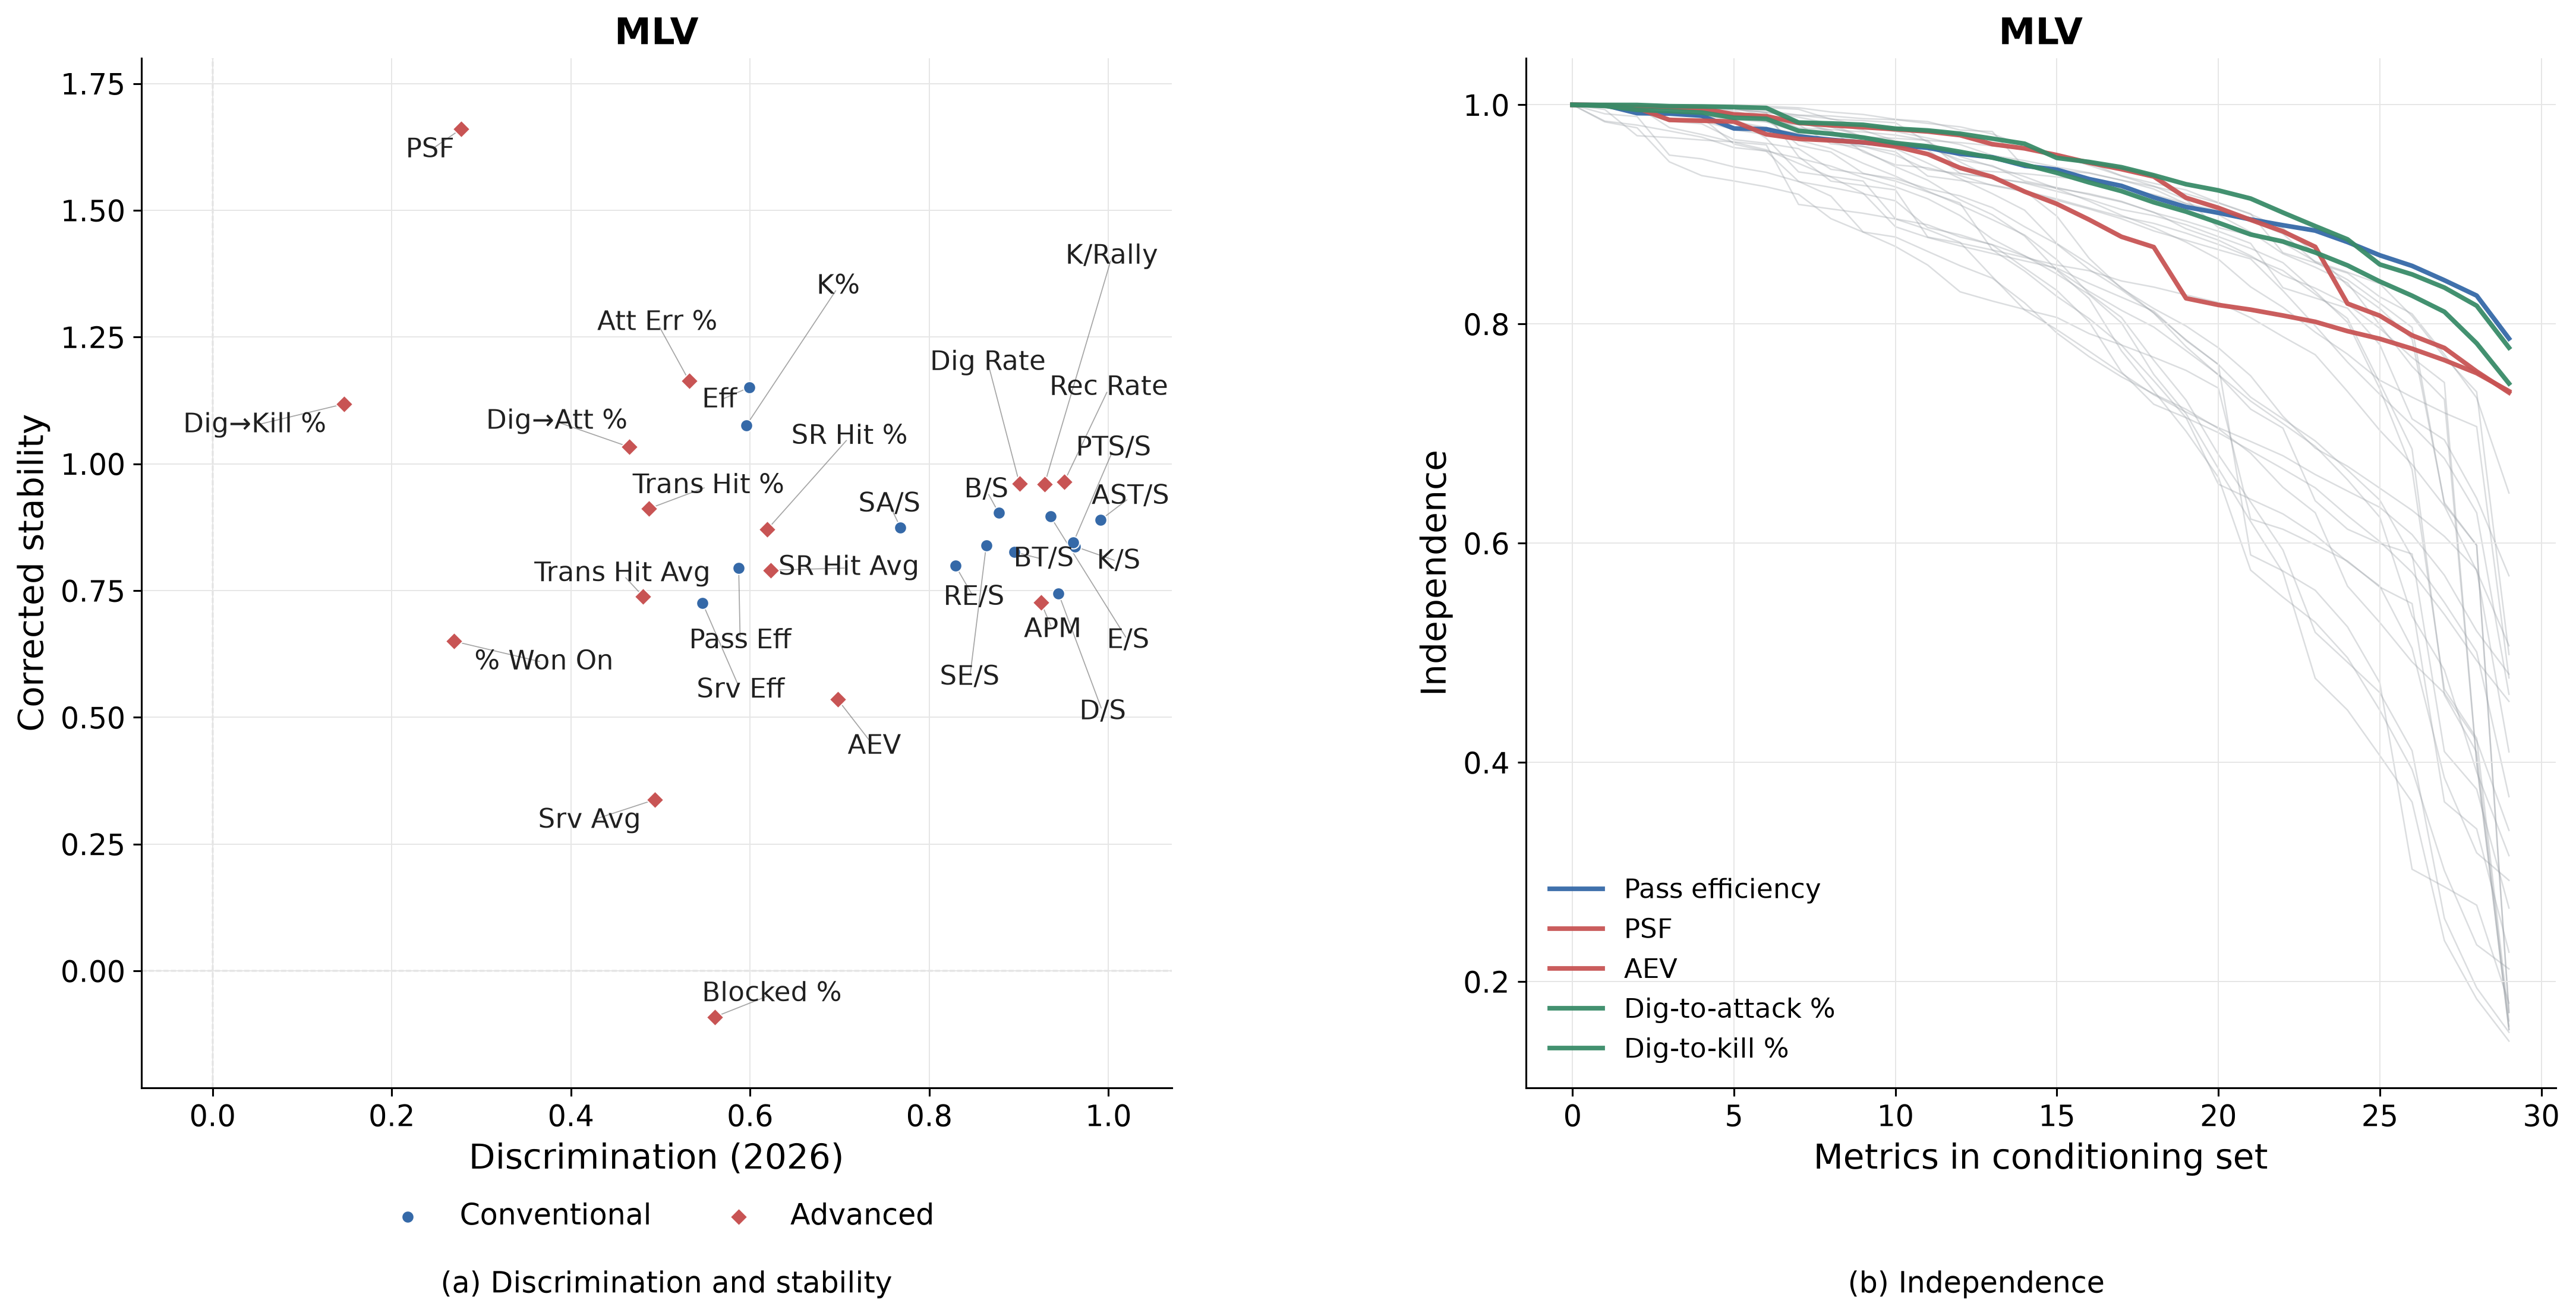
\includegraphics[keepaspectratio]{index_files/figure-latex/notebooks-visualization-fig-meta-mlv-output-2.png}}

}

\caption{\label{fig-meta-mlv}Meta-analytic results for MLV. The left
panel shows latest-season discrimination and corrected stability, with
estimates shown as calculated, including values outside the theoretical
range. The right panel shows the greedy conditional-independence curves,
with the five metrics having the largest full-conditioning independence
values highlighted.}

\end{figure}%

\begin{figure}[H]

\centering{

\pandocbounded{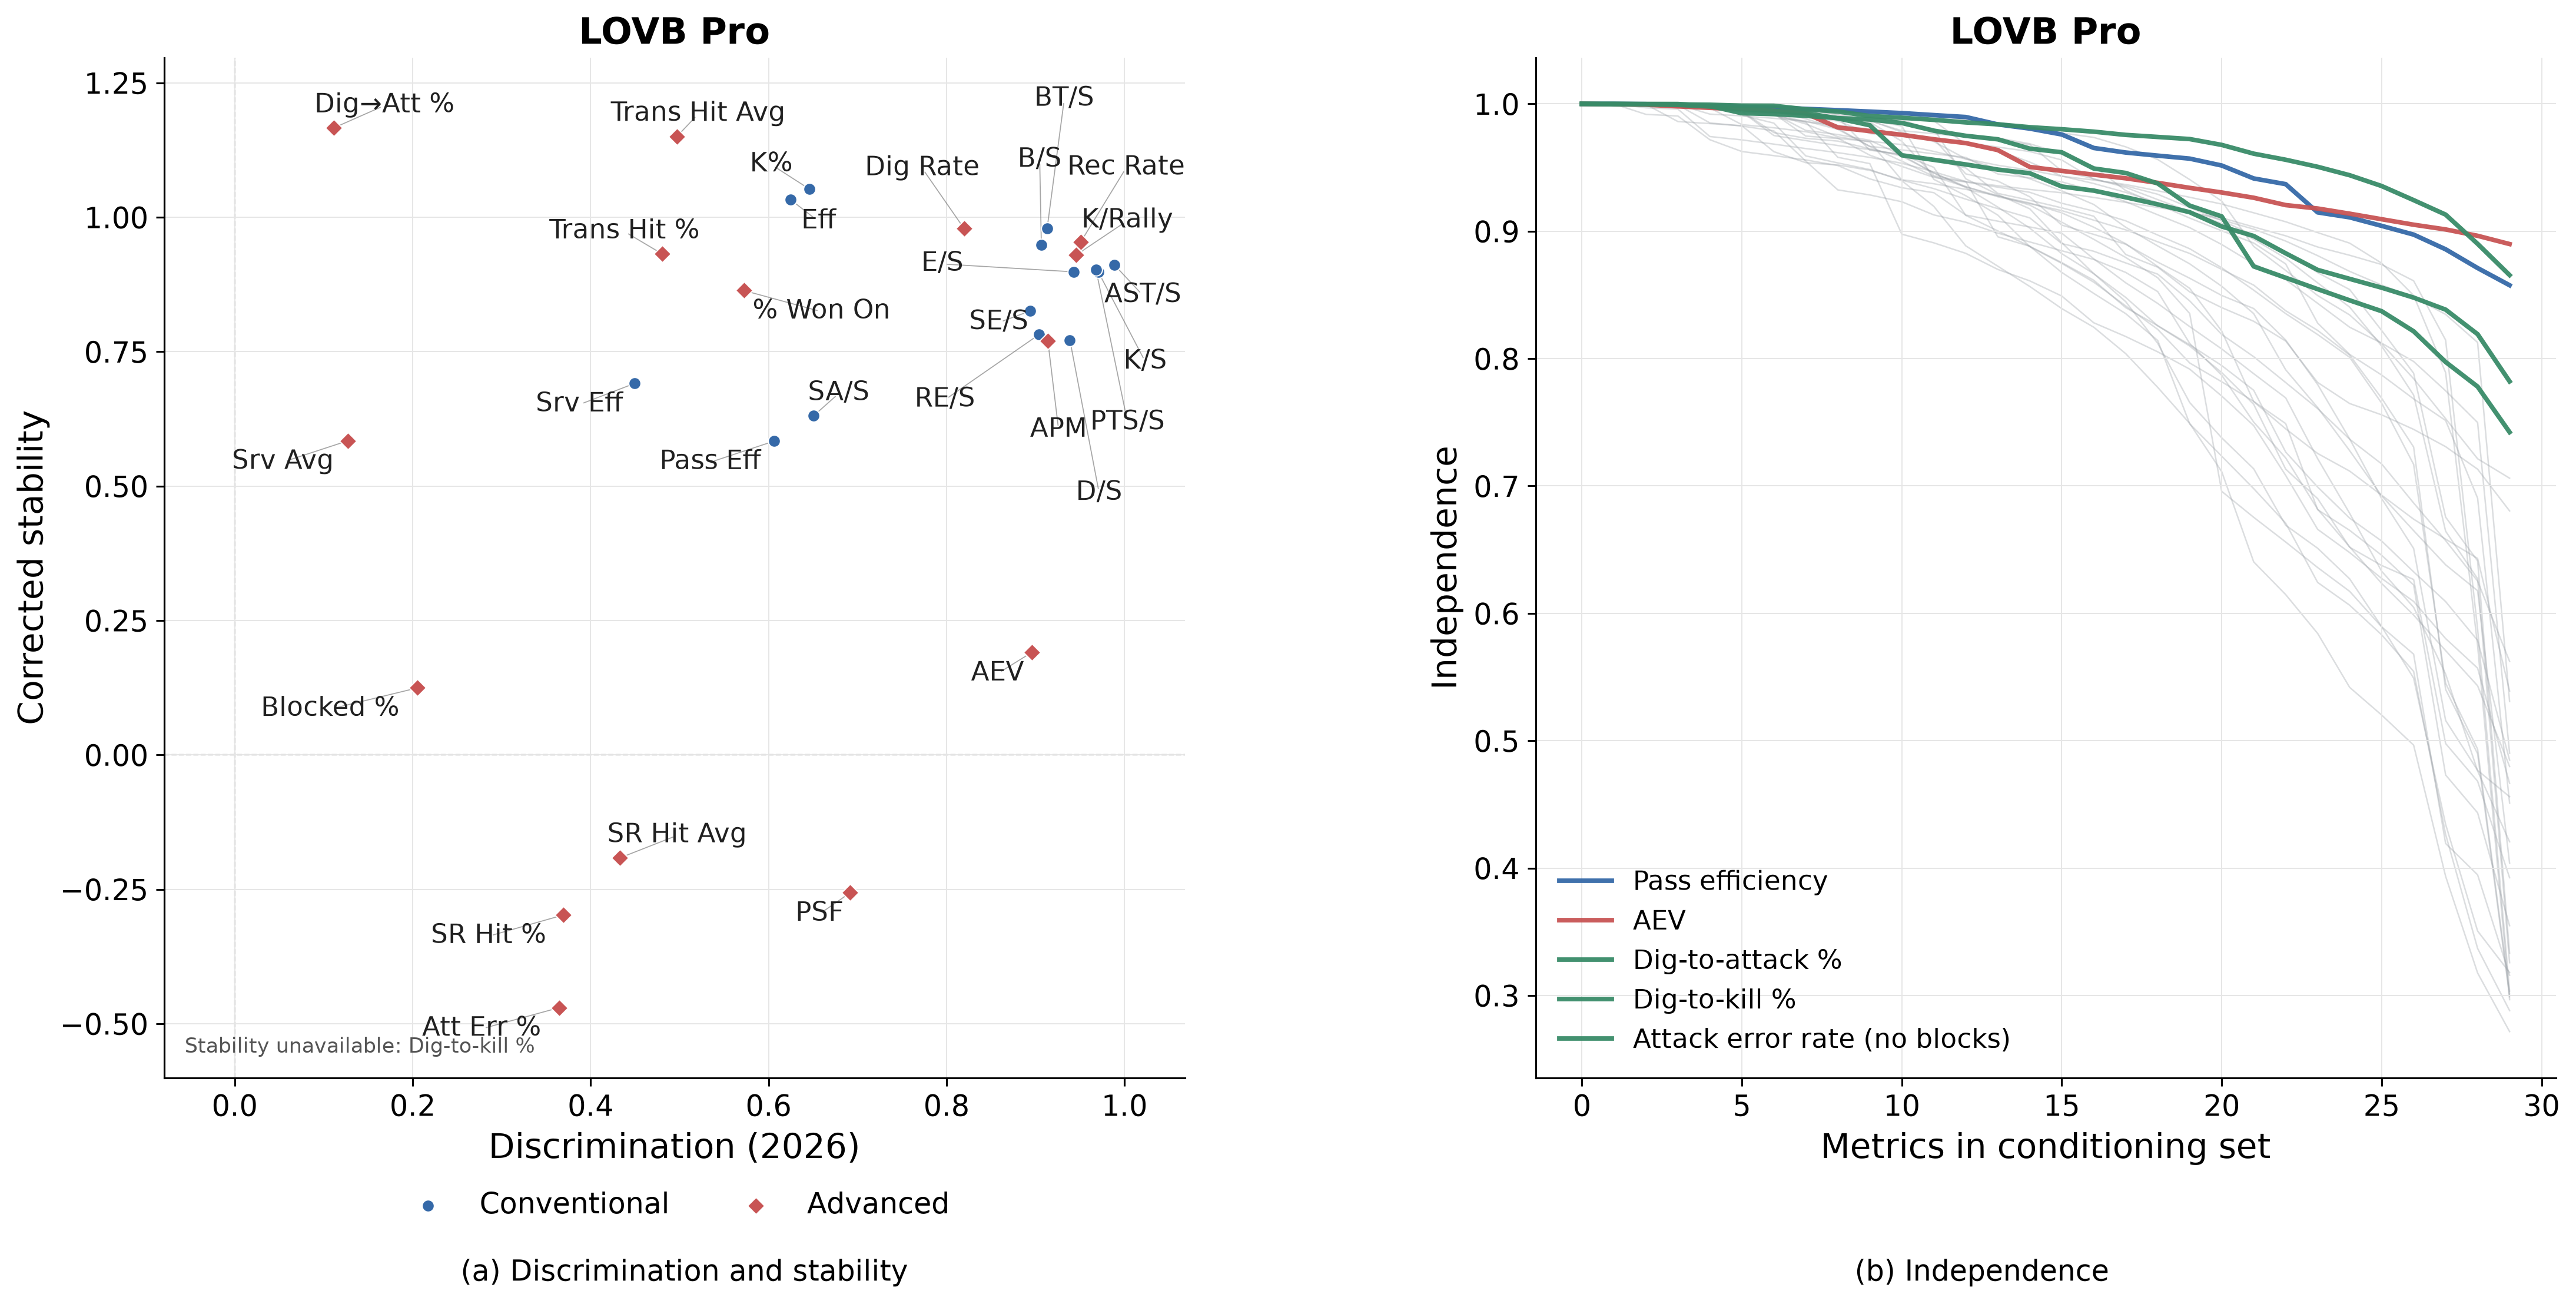
\includegraphics[keepaspectratio]{index_files/figure-latex/notebooks-visualization-fig-meta-lovb-output-1.png}}

}

\caption{\label{fig-meta-lovb}Meta-analytic results for LOVB Pro. The
left panel shows latest-season discrimination and corrected stability,
with estimates shown as calculated, including values outside the
theoretical range. The right panel shows the greedy
conditional-independence curves, with the five metrics having the
largest full-conditioning independence values highlighted.}

\end{figure}%

\begin{figure}[H]

\centering{

\pandocbounded{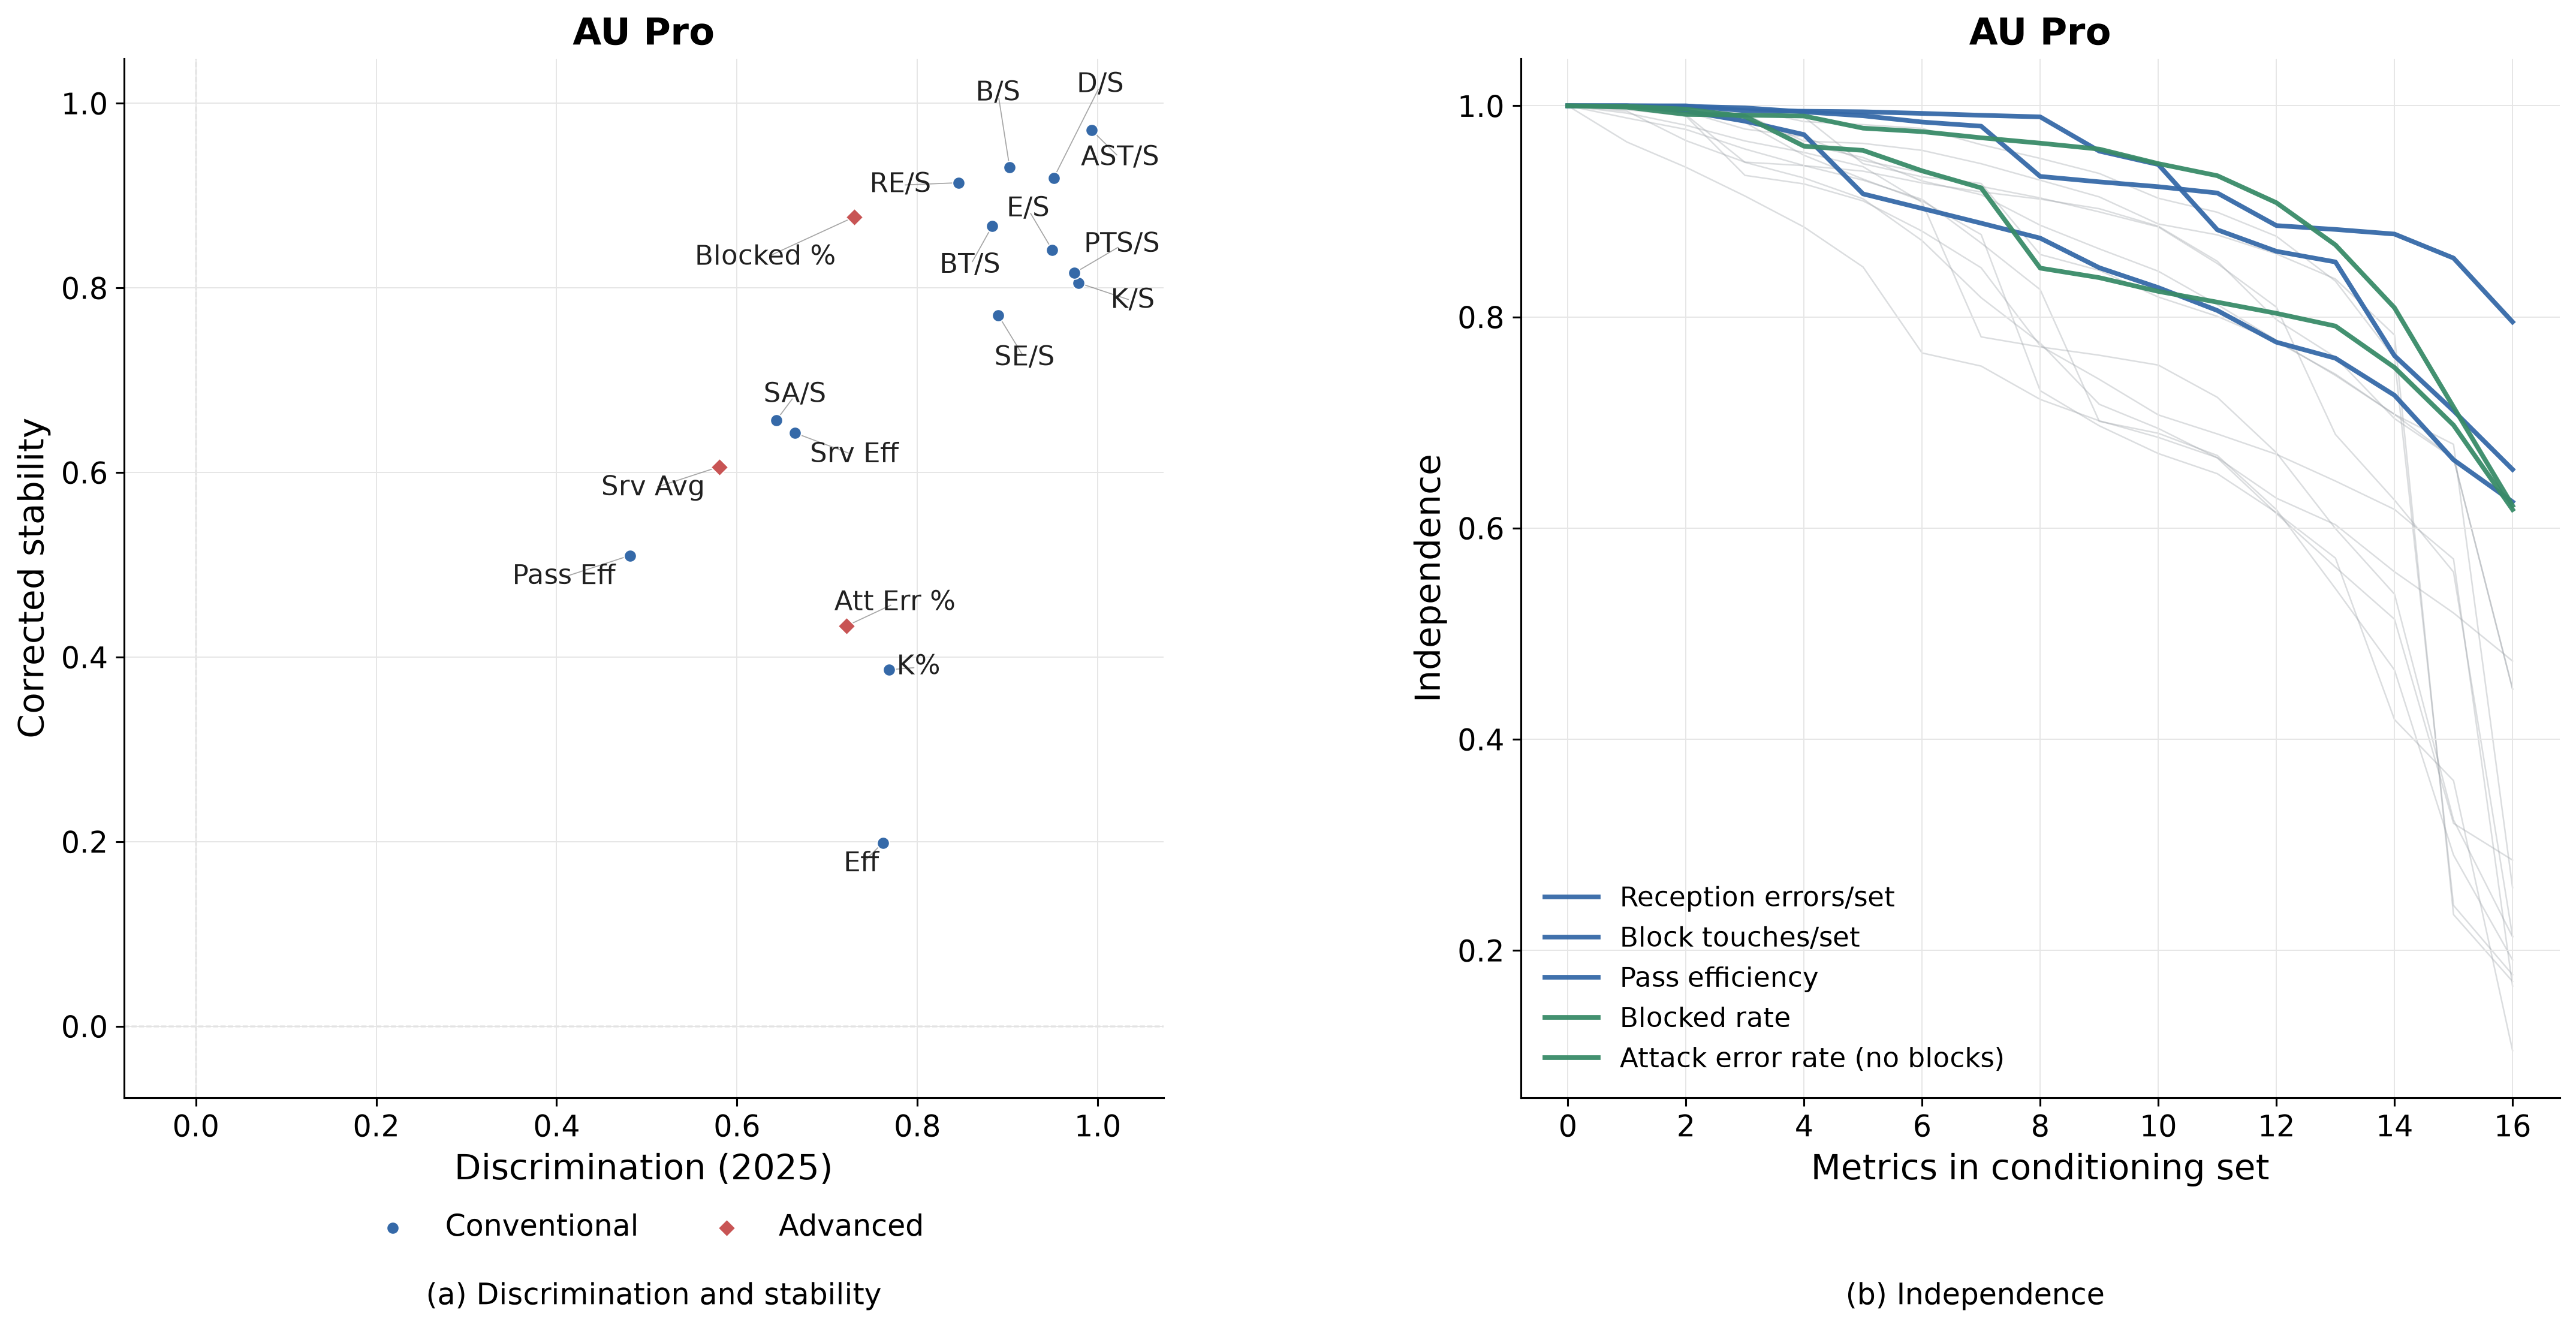
\includegraphics[keepaspectratio]{index_files/figure-latex/notebooks-visualization-fig-meta-au-output-1.png}}

}

\caption{\label{fig-meta-au}Meta-analytic results for AU Pro. The left
panel shows latest-season discrimination and corrected stability. The
right panel shows the greedy conditional-independence curves, with the
five metrics having the largest full-conditioning independence values
highlighted.}

\end{figure}%

\subsection{PCA and Clustering}\label{pca-and-clustering}

Principal component analysis of the latent correlation matrices
indicated substantial but incomplete redundancy among the analyzed
metrics. As shown in Figure~\ref{fig-pca}, MLV required 11, 16, and 21
principal components to explain 80\%, 90\%, and 95\% of latent variance,
respectively. LOVB Pro required 13, 19, and 23 components, while AU Pro
required 7, 10, and 12 components from its smaller 17-metric set.

\begin{figure}[H]

\centering{

\pandocbounded{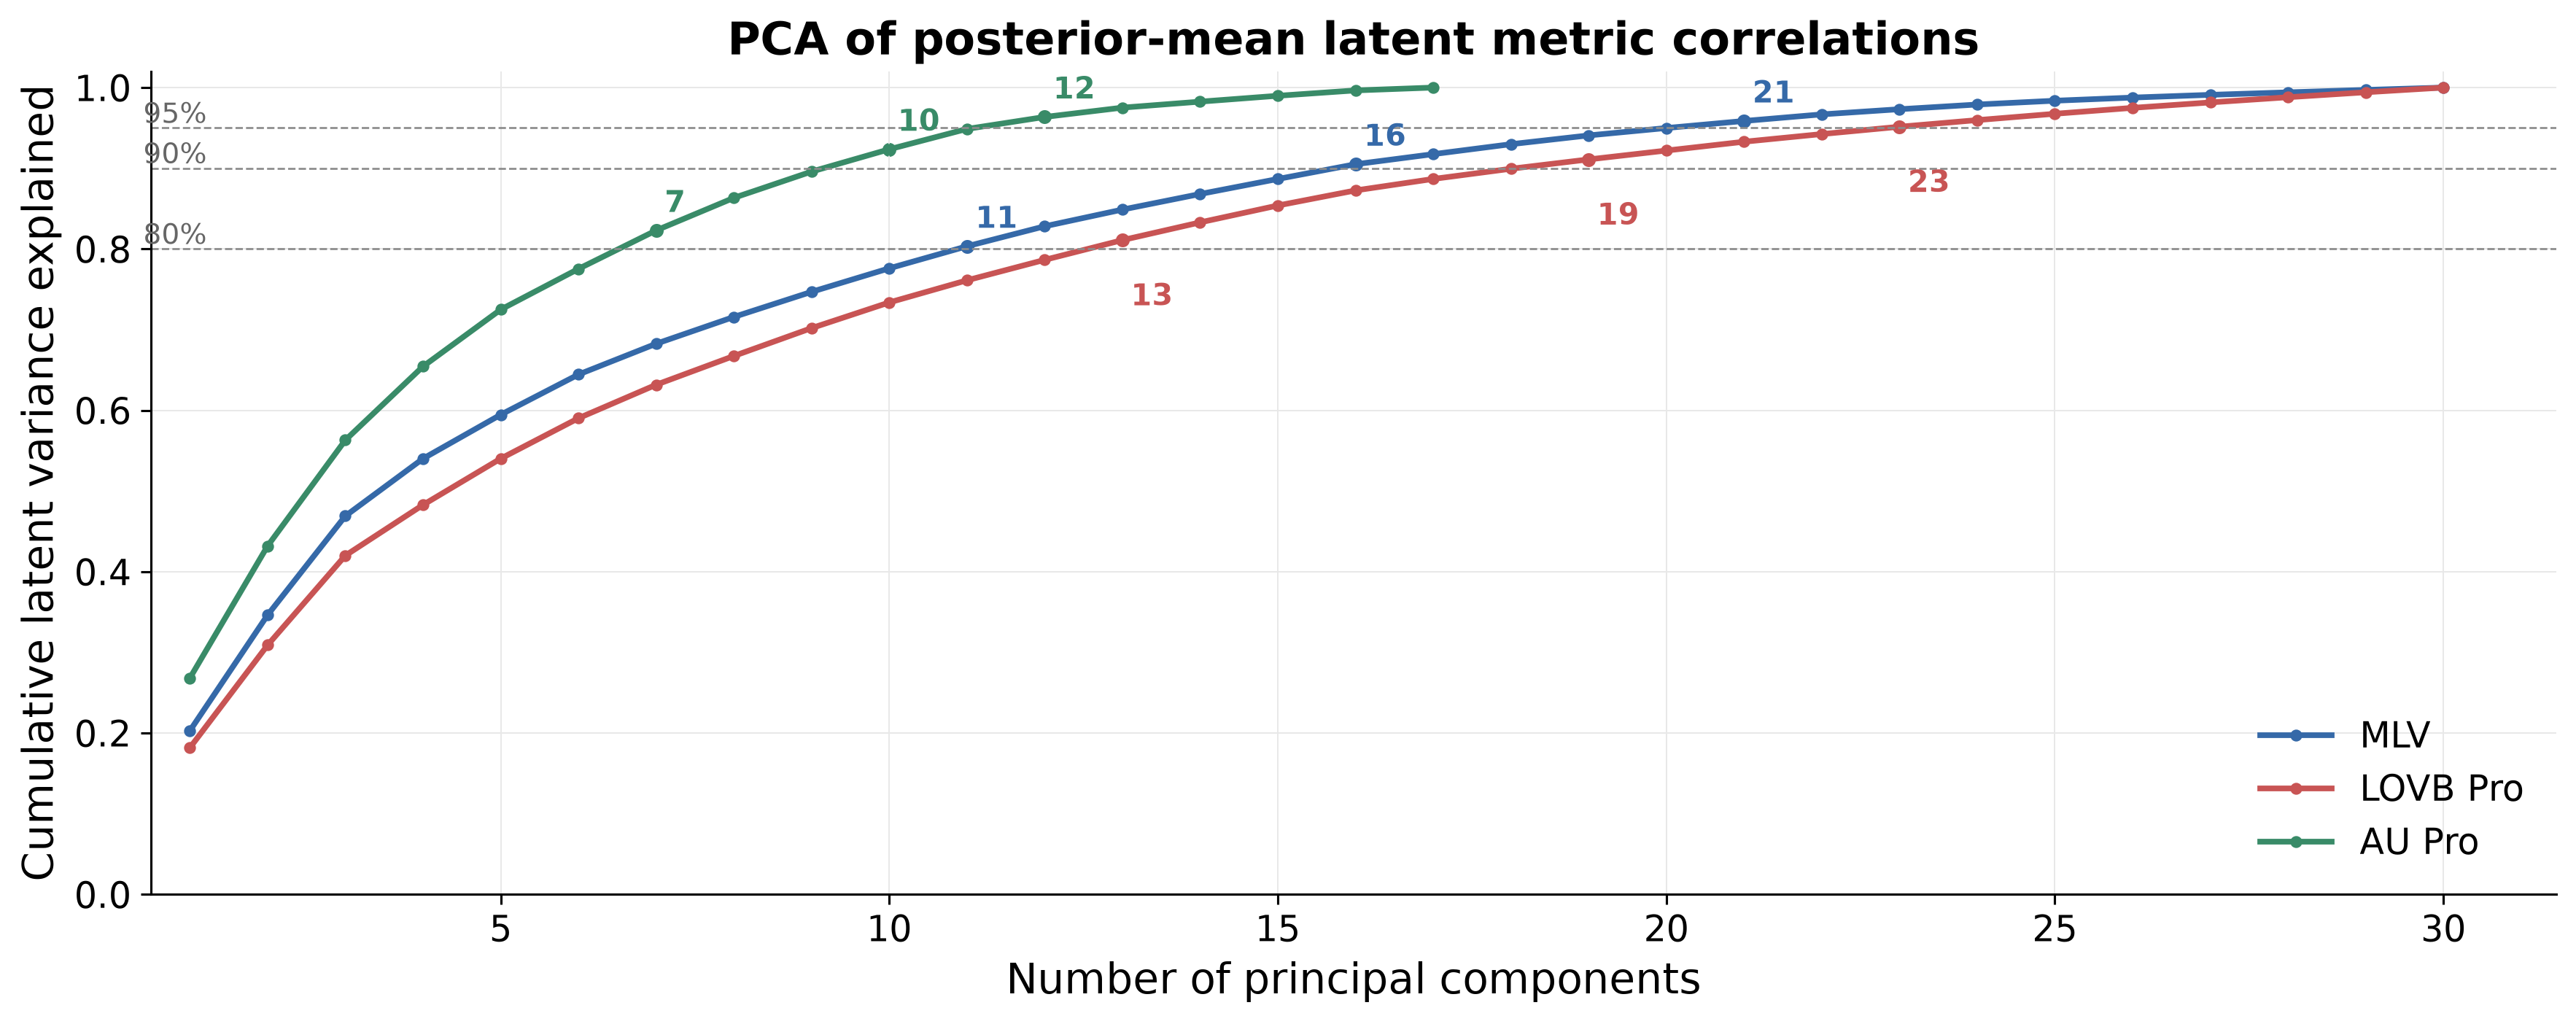
\includegraphics[keepaspectratio]{index_files/figure-latex/notebooks-visualization-fig-pca-output-1.png}}

}

\caption{\label{fig-pca}Cumulative variance explained by principal
components of the posterior-mean latent correlation matrix.}

\end{figure}%

The hierarchical clustering results in
Figure~\ref{fig-clustering-mlv}--Figure~\ref{fig-clustering-au} further
characterize similarities in metric correlation profiles.
\texttt{Kills/set} and \texttt{Points/set} clustered closely in all
three leagues, as did \texttt{Serve\ Average} and
\texttt{Serving\ Efficiency}. In MLV and LOVB Pro,
\texttt{Serve-Receive\ Hit\ Average} clustered closely with
\texttt{Serve-Receive\ Hitting\ Percentage}, while
\texttt{Transition\ Hit\ Average} clustered with
\texttt{Transition\ Hitting\ Percentage}. These clusters reflect
similarity across rows of the absolute latent correlation matrix rather
than only pairwise correlation between the metrics themselves.

\begin{figure}[H]

\centering{

\pandocbounded{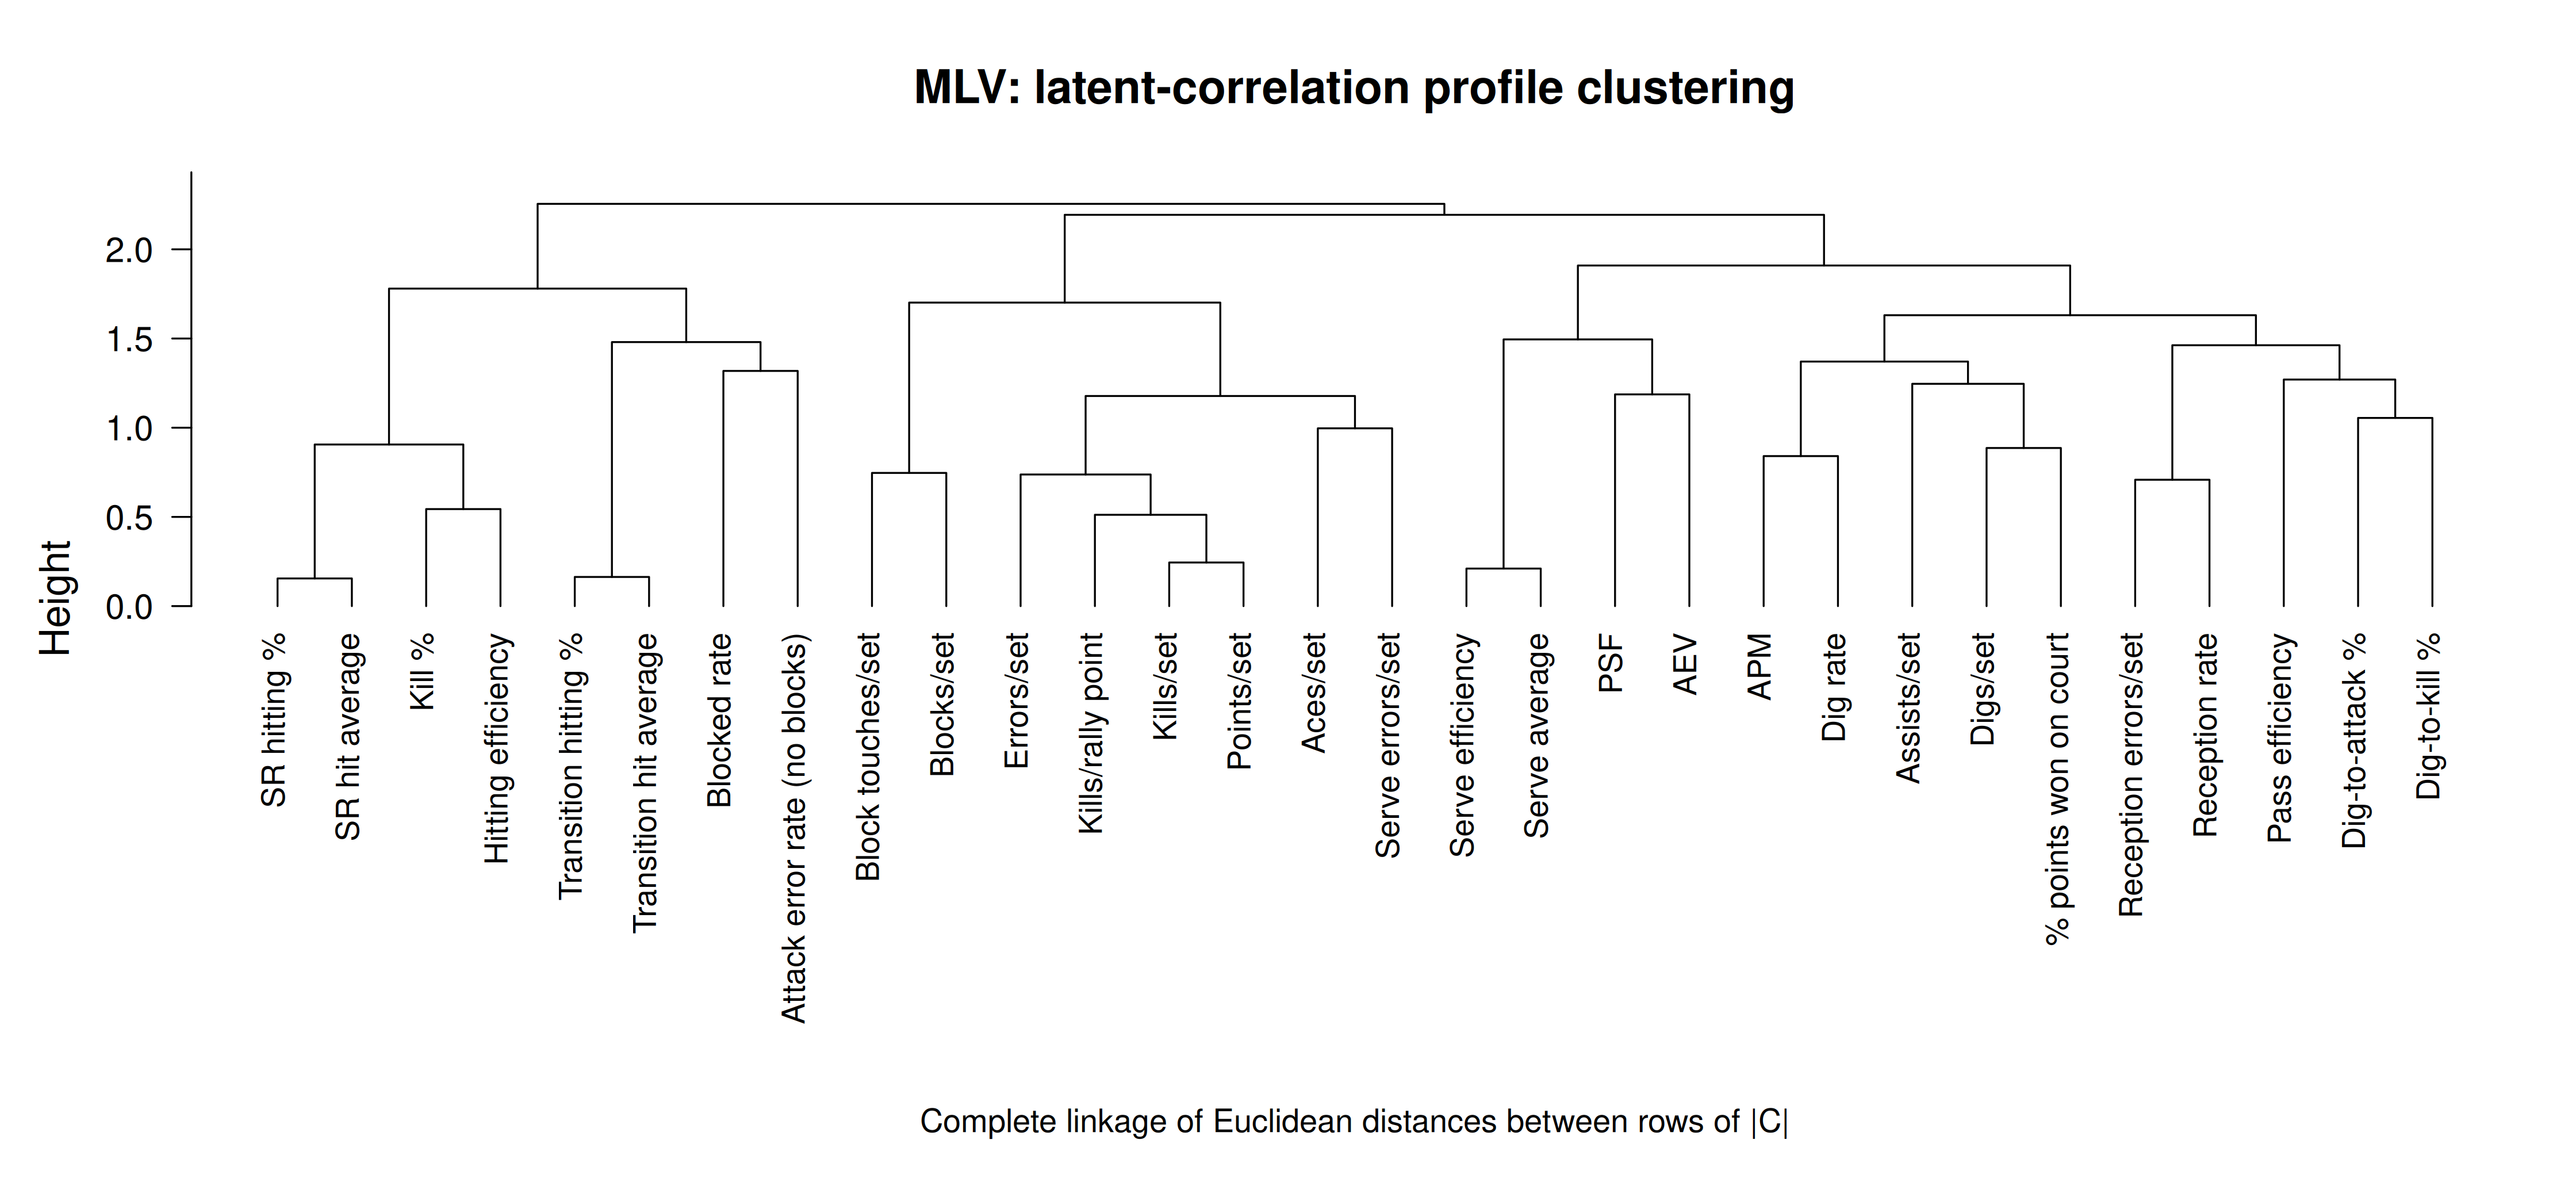
\includegraphics[keepaspectratio]{index_files/figure-latex/notebooks-visualization-fig-clustering-mlv-output-1.png}}

}

\caption{\label{fig-clustering-mlv}Complete-linkage hierarchical
clustering of metric correlation profiles for MLV. Distances are
Euclidean distances between rows of the absolute posterior-mean latent
correlation matrix.}

\end{figure}%

\begin{figure}[H]

\centering{

\pandocbounded{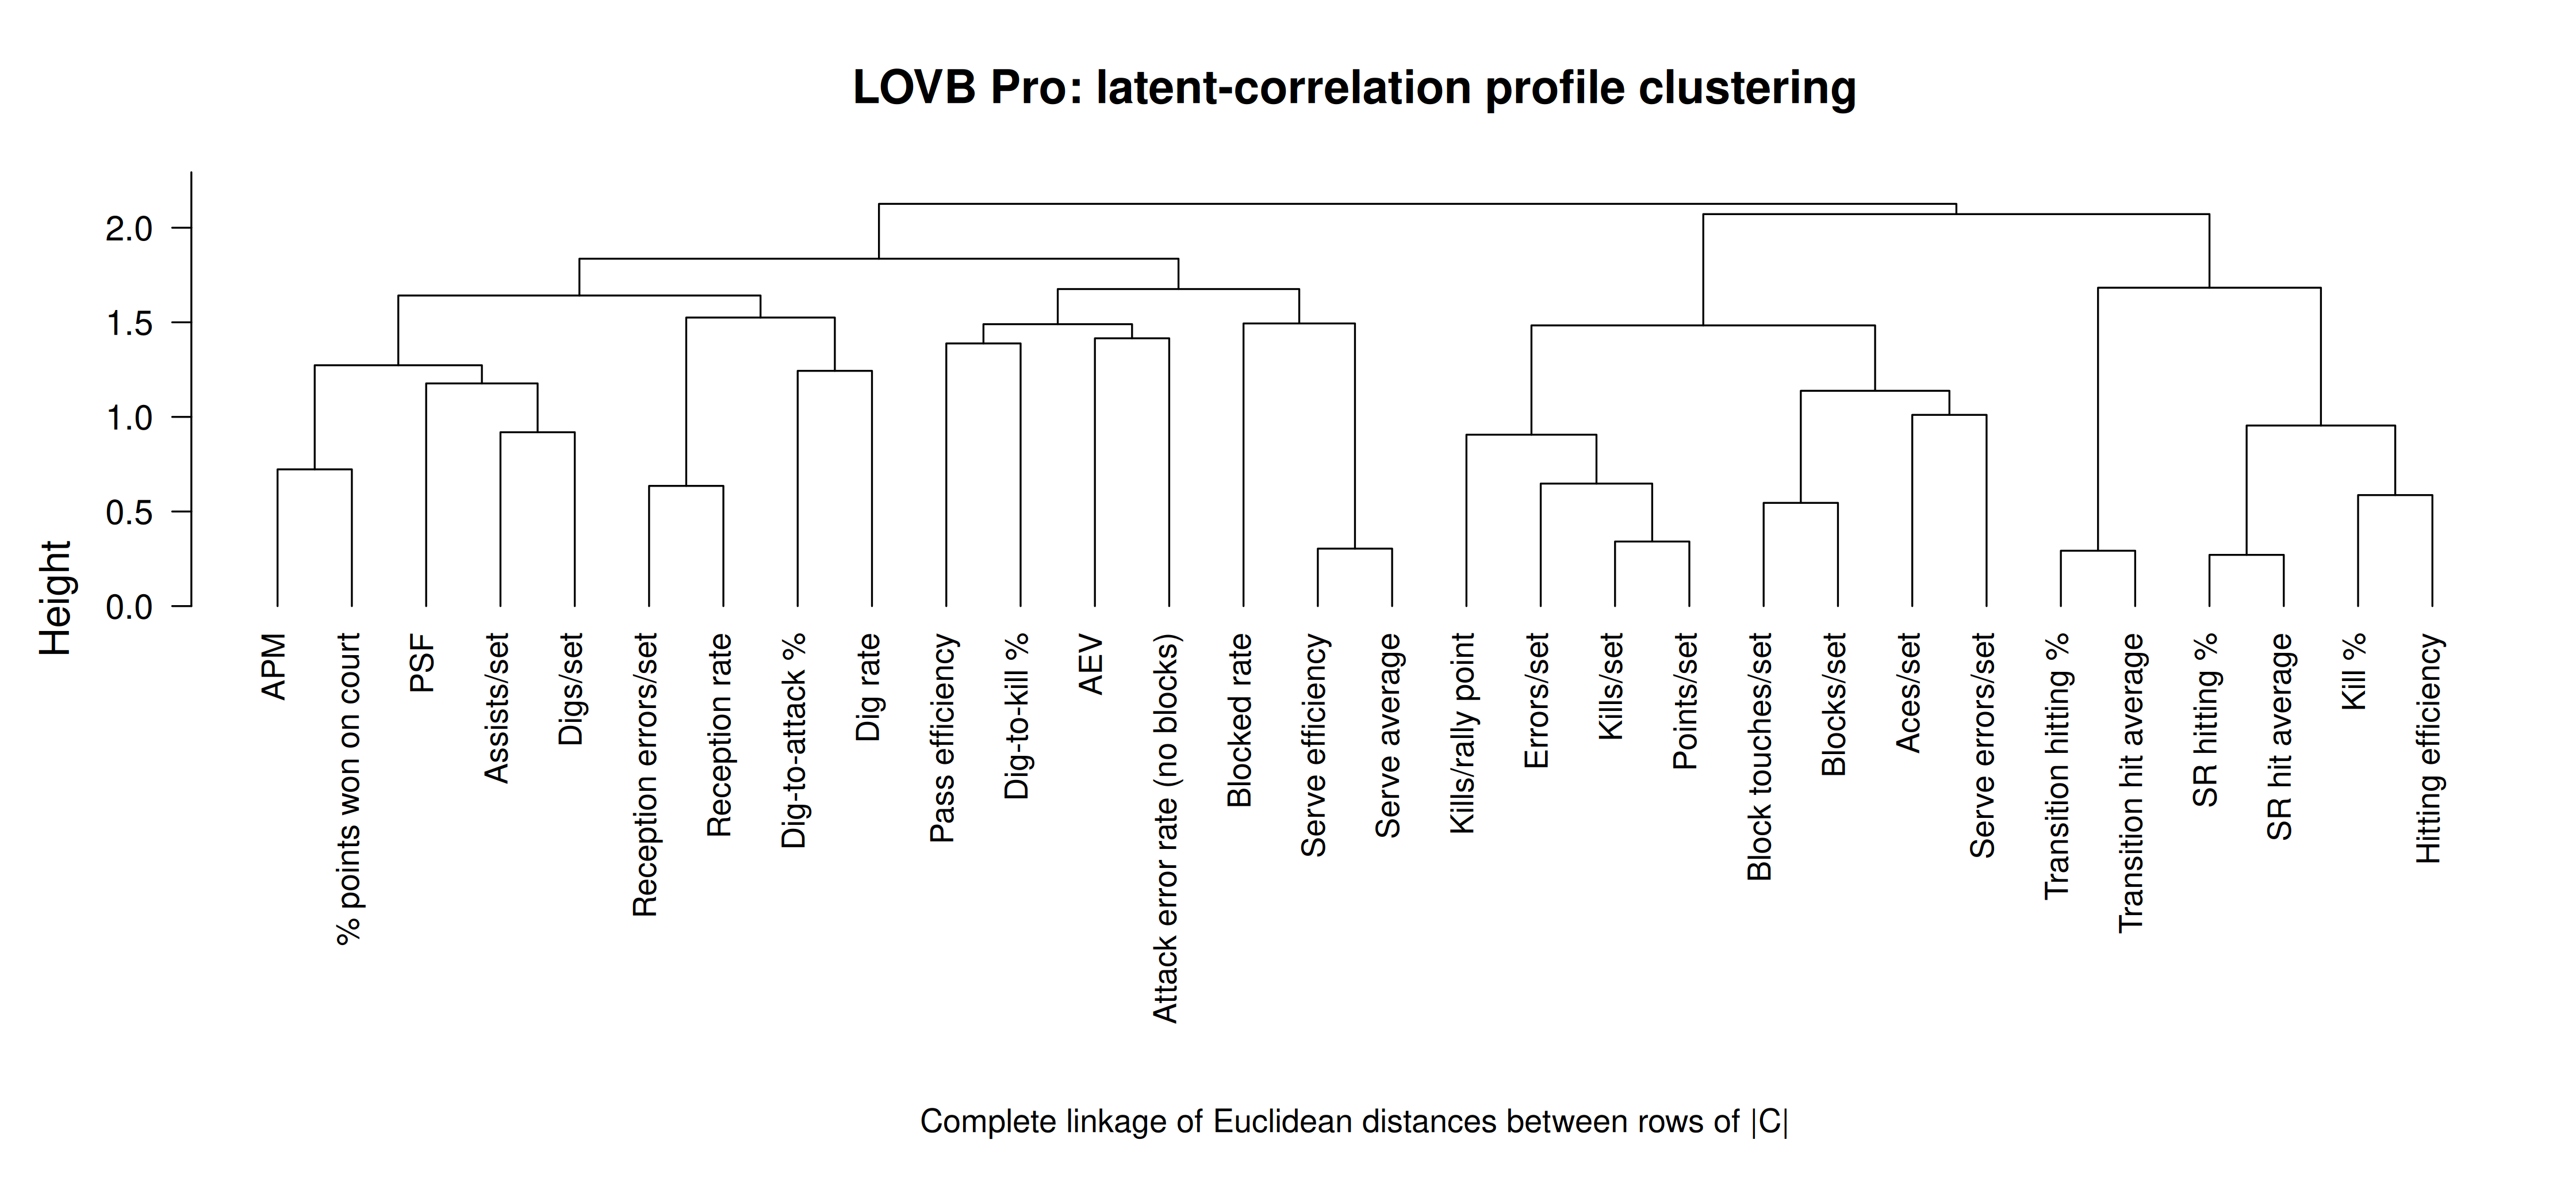
\includegraphics[keepaspectratio]{index_files/figure-latex/notebooks-visualization-fig-clustering-lovb-output-1.png}}

}

\caption{\label{fig-clustering-lovb}Complete-linkage hierarchical
clustering of metric correlation profiles for LOVB Pro. Distances are
Euclidean distances between rows of the absolute posterior-mean latent
correlation matrix.}

\end{figure}%

\begin{figure}[H]

\centering{

\pandocbounded{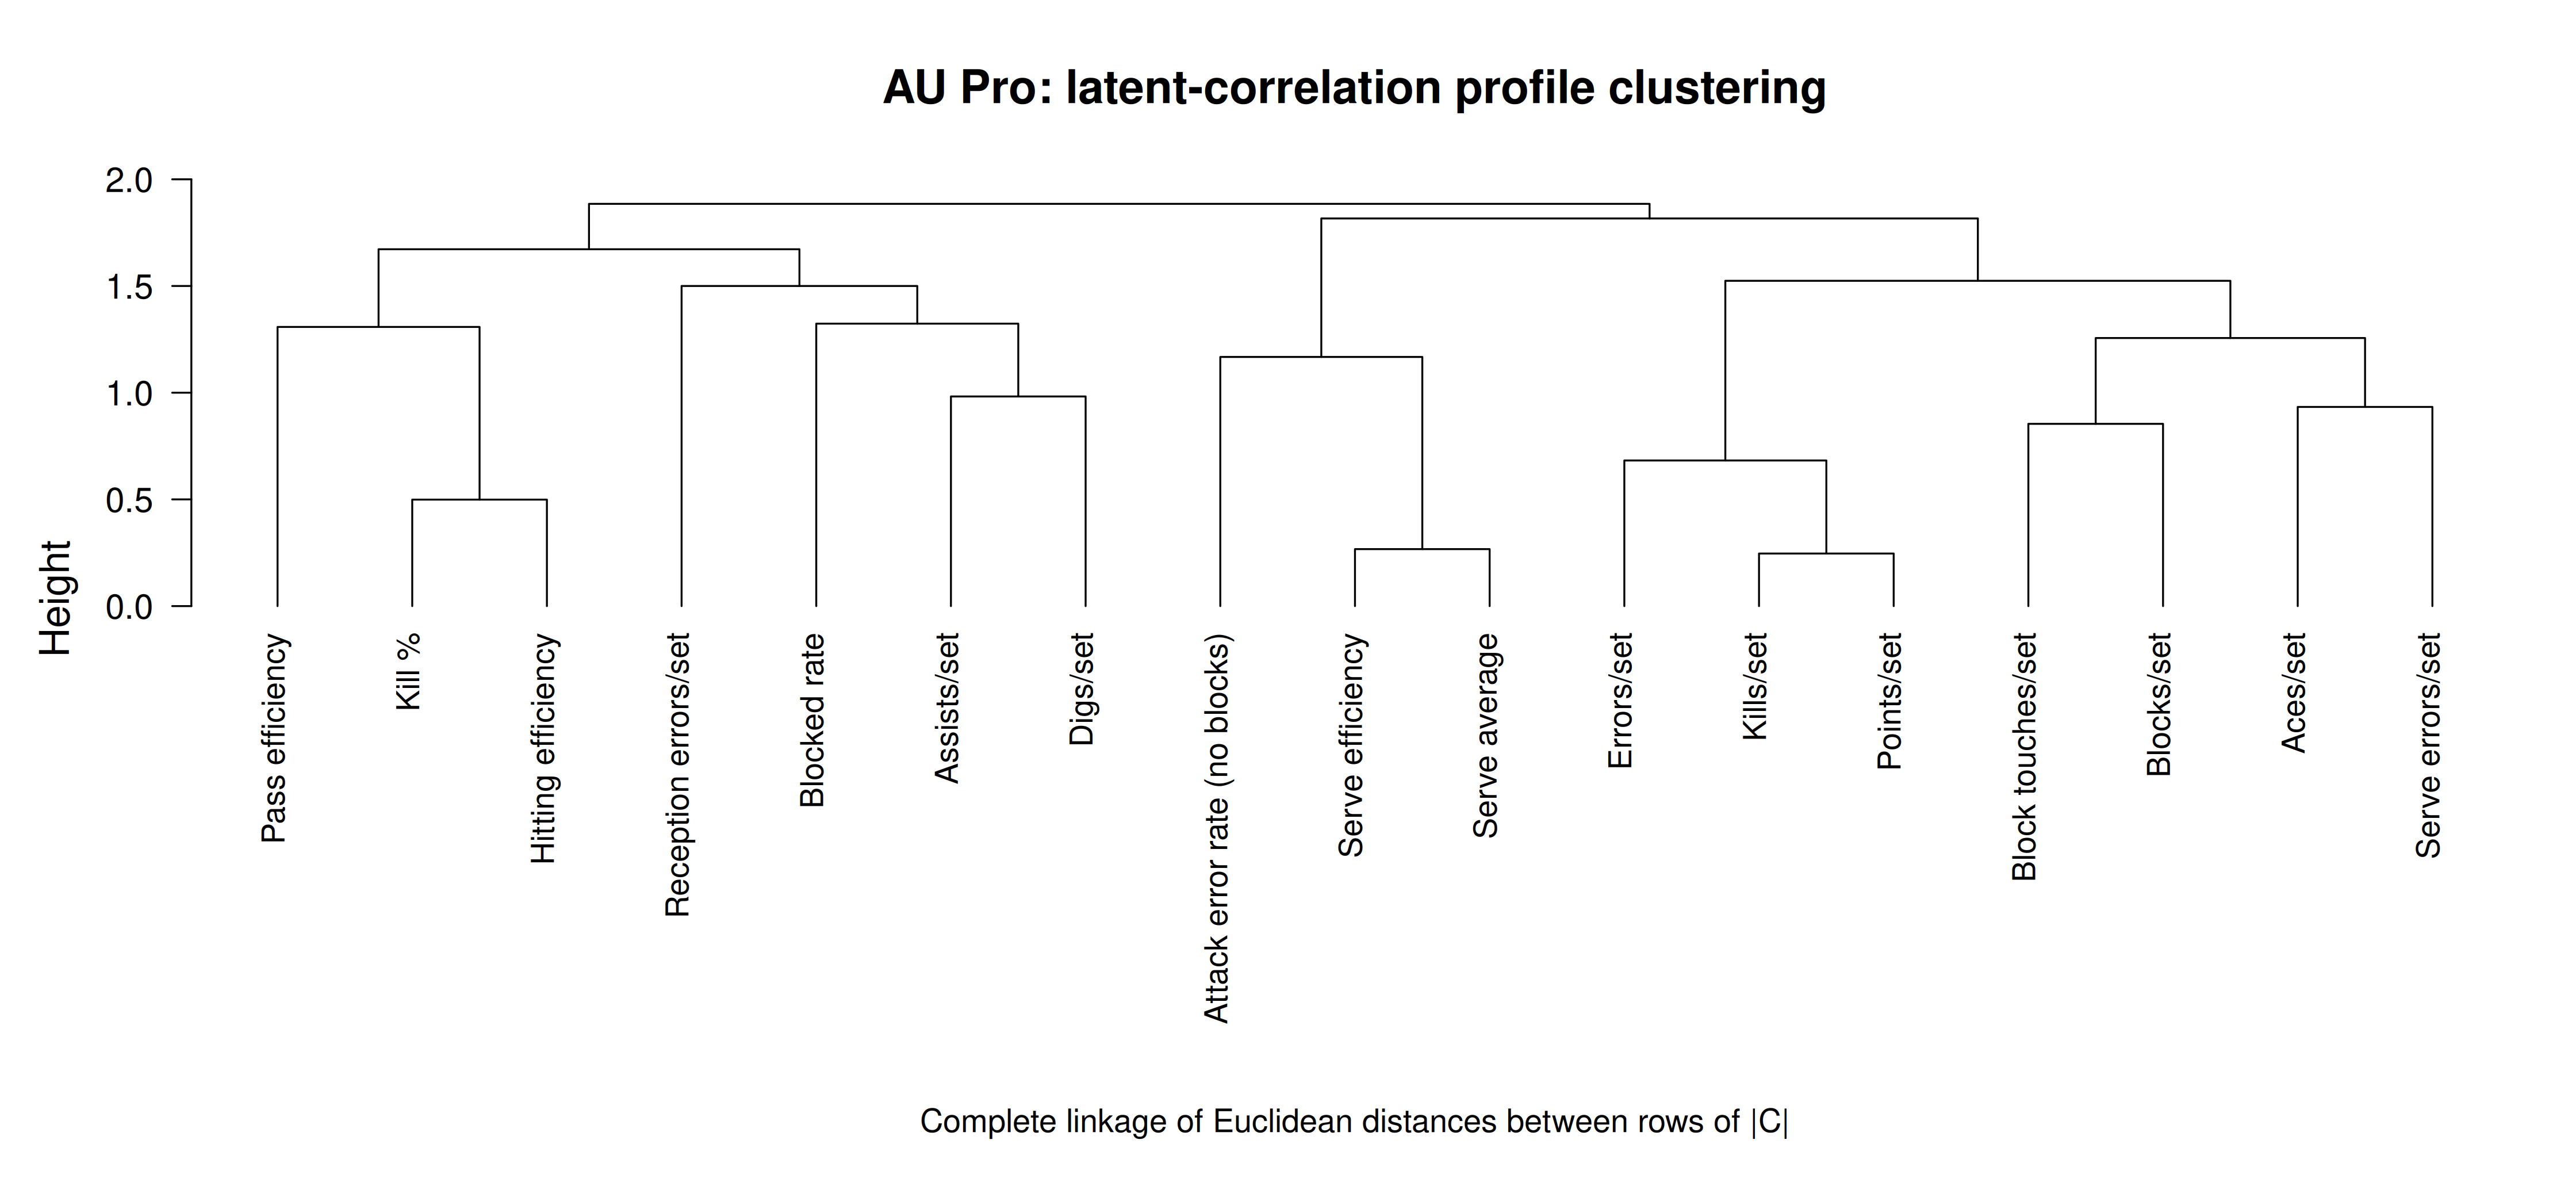
\includegraphics[keepaspectratio]{index_files/figure-latex/notebooks-visualization-fig-clustering-au-output-1.png}}

}

\caption{\label{fig-clustering-au}Complete-linkage hierarchical
clustering of metric correlation profiles for AU Pro. Distances are
Euclidean distances between rows of the absolute posterior-mean latent
correlation matrix.}

\end{figure}%

\section{Discussion}\label{discussion}

The results demonstrate that meta-metrics capture distinct properties of
volleyball metrics and should therefore be considered jointly. Several
conventional per-set statistics, particularly \texttt{Assists/set},
\texttt{Kills/set}, and \texttt{Points/set}, were highly discriminative
across leagues but were also among the least independent metrics.
Conversely, advanced metrics such as \texttt{AEV} and the dig-conversion
measures contributed comparatively distinct information despite lower
discrimination or stability in some settings. A metric can therefore
distinguish players clearly without adding much new information, or
provide comparatively non-redundant information while remaining
sensitive to sampling variability or season-to-season change. The
cross-league results further demonstrate that these statistical
properties are not necessarily intrinsic to the metric itself: although
some discrimination patterns were consistent, stability differed
considerably across MLV, LOVB Pro, and AU Pro. For example, \texttt{PSF}
had a large corrected stability estimate in MLV but a negative estimate
in LOVB Pro. Such differences may reflect variation in player
populations, season length, player movement, competitive structure,
opportunity distributions, or available data, and a metric that behaves
reliably in one competition should not automatically be assumed to have
the same properties in another.

PCA and clustering reinforce the distinction between redundancy and
unique information. Although the original set of metrics could be
reduced, several principal components were still needed to capture most
of the variation, suggesting that the metrics reflected more than just a
few common underlying patterns. At the same time, intuitive clusters
such as \texttt{Kills/set} with \texttt{Points/set} and
\texttt{Serve\ Average} with \texttt{Serving\ Efficiency} identify
groups of statistics that may provide overlapping descriptions of player
performance. These properties have direct applications when deciding
which statistics to communicate to practitioners. In a scouting report,
discrimination and stability can help identify metrics that provide
comparatively reliable separation between players, while independence
can help avoid presenting several statistics that largely repeat the
same underlying information. A report could therefore prioritize a
smaller collection of complementary metrics rather than simply including
every available statistic. Similarly, coaches could use reliable
skill-specific measures to monitor areas of player performance that have
already been identified as priorities. Meta-analytic evaluation does not
tell coaches which training plan to use, but it can help guide the
selection and monitoring of metrics that are reliable and informative
enough to interpret meaningfully.

\section{Conclusion}\label{conclusion}

This study applies a meta-analytic framework to evaluate the statistical
properties of conventional and advanced player-performance metrics
across professional women's volleyball leagues. The results demonstrate
that discrimination, stability, and independence provide complementary
perspectives on metric quality, with no single property sufficient to
characterize a metric on its own. Several conventional per-set
statistics clearly distinguish between players but also contain
substantial overlap with other measures, while some advanced metrics
provide comparatively non-redundant information despite weaker
discrimination or stability. These results are echoed via principal
components analysis and hierarchical clustering. Differences across
leagues further demonstrate that the statistical behaviour of a metric
depends in part on the competition, available data, and player
population in which it is evaluated. Together, these findings show that
the growing number of volleyball metrics should not be interpreted
solely according to their definitions or apparent complexity, but also
according to the statistical information they provide. For
practitioners, meta-analytic evaluation can help support the selection
of smaller and more complementary sets of statistics for scouting,
player development, and performance communication. More broadly, this
work provides a systematic and applied framework for evaluating existing
and proposed volleyball metrics.

\subsection{Limitations and Future
Work}\label{limitations-and-future-work}

Several limitations should be considered when interpreting these
results. Only a small number of seasons are available for each
professional competition, leaving many repeated players with two or
three qualifying seasons and limiting the precision with which stability
can be estimated. Advanced measures requiring detailed sequence or
lineup information also have more restricted coverage, and \texttt{AEV}
in particular is available for relatively few player-seasons because of
its setter and attack-volume requirements. Player specialization and
differences in opportunity may additionally contribute to some of the
observed statistical properties because players in different roles are
exposed to substantially different actions and responsibilities.

Future work can revisit these analyses in later years as these
relatively nascent leagues continue to mature and grow. Larger
repeated-player populations would allow stability to be estimated more
precisely, while improved data coverage would support more consistent
evaluation of advanced metrics across leagues. A second direction is to
expand the set of metrics included in the analysis as research in the
volleyball analytics space develops. This would provide a more complete
picture of which aspects of volleyball performance are already well
represented and where meaningful gaps remain. The identified gaps can in
turn inform the development of new volleyball metrics. Position-specific
meta-analytics represents another important extension because volleyball
roles differ substantially in both responsibilities and statistical
opportunities. Evaluating setters, hitters, middle blockers, liberos,
and other positional groups separately could help distinguish properties
of the metrics themselves from patterns driven primarily by role and
opportunity. The framework could also be extended beyond professional
volleyball to collegiate leagues such as NCAA and U SPORTS volleyball.
This would provide larger and structurally different player populations
from which patterns observed across professional leagues can be
identified earlier on in a player's career. Finally, meta-analytic
properties could be considered alongside predictive or decision-specific
objectives. Discrimination, stability, and independence do not directly
measure predictive value or causal contribution to winning, so future
work could separately evaluate how metrics with different meta-analytic
profiles relate to outcomes such as point, set, or match success and to
specific scouting or coaching decisions.

\section*{References}\label{references}
\addcontentsline{toc}{section}{References}

\renewcommand{\bibsection}{}
\bibliography{references.bib}





\end{document}
